\documentclass[t]{beamer}
\usetheme{Warsaw}
\usepackage{array}
\usecolortheme{seahorse}
%\usepackage{graphicx}
\usepackage{amssymb,amsmath,mathrsfs,amsfonts}
%\usepackage[colorhighlight,display]{texpower}
%\usepackage{caption}
%\usepackage[all]{xy}
\usepackage{beamerthemesplit}
\mode<presentation>
%\usepackage{pause}
\usepackage{ulem}  % for strikethroughs
\usepackage{cancel} % for strikethroughs in math mode 
\usepackage{tikz}
\usetikzlibrary{shapes}
\usepackage{hyperref}
\hypersetup{pdfpagemode=FullScreen}
\usepackage{ifthen}
\usepackage{animate}
\usepackage{color}
\usepackage{type1cm}  % used for watermarking
\usepackage{eso-pic}  % used for watermarking



\theoremstyle{plain}
\newtheorem{prop}{Proposition}
\newtheorem{thm}[prop]{Theorem}
\newtheorem{lem}[prop]{Lemma}
\newtheorem{cor}[prop]{Corollary}
\theoremstyle{definition}
\newtheorem{dfn}{Definition}
\newtheorem{rem}[prop]{Remark}
\newtheorem{ex}{Example}[section]
%\newtheorem{note}{Note}[section]
\newtheorem{exercise}{Exercise}[section]
\newcommand{\nin}{\noindent}
\newcommand{\ds}{\displaystyle}
\renewcommand{\figurename}{Figure \arabic{figure}}



\renewcommand*\familydefault{\sfdefault} 




%%%%%%%%%%%%%%%%%%%%%%%%%%5
%%%%%%%%%%%%%%%%%%%%%%%%%%%%
%%%% some commands that have different meaning in the article/presentation modes

\newcommand{\vvfill}{\mode<presentation>{\vfill}  \mode<article>{\medskip}}   %vfill in presentation only
\newcommand{\sketchspace}{ 
\mode<article>{ \medskip\noindent{\textbf{Sketch:}} \vspace*{6cm} }
\mode<presentation>{ } 
}
\newcommand{\examplespace}{ 
\mode<article>{ \medskip\noindent{\textbf{Example:}} \vspace{6cm} }
\mode<presentation>{ } 
}
\newcommand{\artsmspace}{\mode<article>{\vspace*{2cm}} }  %small space in article mode
\newcommand{\artlargespace}{\mode<article>{\vspace*{6cm}} }  %large space in article mode

\newcommand{\dx}{\,dx}

\newcommand{\soln}{{\textbf{Solution: }}\,\,\,}


\newcommand{\makedate}{\vvfill
\begin{picture}(10,10)  
\put(260,-20){\mbox{\tiny{\today}}}
\end{picture}
}

\newcommand{\pd}[2]{\dfrac{\partial#1}{\partial#2}}
\newcommand{\pD}[2]{\dfrac{\partial^2#1}{\partial#2^2}}
\newcommand{\pdd}[3]{\dfrac{\partial^2#1}{\partial#2 \partial#3}}


\normalem %stops the ulem package making all the emphs into underlines....
 
 
 
 \newcommand{\refandrev}[2]{
 \begin{small}
  \hspace{6cm}
  \begin{minipage}[r]{8cm}
  Stewart,    Chapter #1   \\
  Review:  \parbox[t]{6cm}{#2}
\end{minipage}
\end{small}
}



\newcounter{heading}
\setcounter{section}{1}
\setcounter{heading}{0}

\newcommand{\makeheading}[1]{\medskip\begin{large}\noindent\textbf{{#1}}\end{large}\smallskip}

%\newenvironment{head}[1]{\medskip\stepcounter{heading}\noindent\textbf{\hspace{0.2cm}{#1}.}}{}
\newcommand{\newhead}[1]{\medskip\stepcounter{heading}\noindent\textbf{\hspace{0.2cm}{#1}.}}


\newcommand{\pf}[1]{\noindent\textit{Proof.}\vspace*{#1 cm}}
\newcommand{\sol}[1]{\noindent\textit{Solution.}\vspace*{#1 cm}}
\newcommand{\further}[1]{\begin{small}\noindent\textit{Further reading: #1}\end{small}}
\newcommand{\exr}[1]{\begin{footnotesize}\noindent\textit{\textbf{Exercises:} Stewart #1}\end{footnotesize}}


% Sets of numbers
\newcommand{\C}{\mathbb{C}}
\newcommand{\RR}{\mathbb{R}}
\newcommand{\Z}{\mathbb{Z}}
\newcommand{\N}{\mathbb{N}}
\newcommand{\Q}{\mathbb{Q}}

% Partitions
\newcommand{\PP}{\mathcal{P}}

% Limits
\newcommand{\limm}[1]{\displaystyle \lim_{x\to #1}}

% Backslash
\newcommand{\bs}{\backslash}

% functions
\newcommand{\cosec}{\mathrm{cosec}}
\newcommand{\cosech}{\mathrm{cosech}}
\newcommand{\sech}{\mathrm{sech}}
\newcommand{\Li}{\mathrm{Li}}
\newcommand{\si}{\mathrm{Si}}
\newcommand{\erf}{\mathrm{erf}}

% Domain and Range
\newcommand{\Dom}{\mathrm{Dom}}
\newcommand{\Codom}{\mathrm{Codom}}
\newcommand{\Range}{\mathrm{Ran}}



\title{Week 1:   Functions}
%\date{July 23 -- July 27, 2012}

\begin{document}

\frame{\titlepage}

\setcounter{tocdepth}{2}
\frame{\tableofcontents
} 

\AtBeginSection[]
{
\begin{frame}<beamer> 
\tableofcontents[currentsection]  % show TOC and highlight current section
\end{frame}
}


\frame
{
\frametitle{Administration}
\begin{itemize}
\setlength{\itemindent}{.5in}
\item[Name] Chaklam Silpasuwanchai
\item[Email] chaklam@ait.asia
\item[Website] \url{http://chaklam.com}
\item[Textbook] Thomas Calculus 13 ed., Stewart Calculus 8 ed.
\item[GClassroom] ahh7xn4
\item[Grade] Midterm 35 Final 35 Quizzes 30
%\item[URL] {\small\url{http://maths.anu.edu.au/~banerjee/Math1014notes.html}}
\end{itemize}}

\section{Introduction}
\subsection{Sets}
\begin{frame}
\footnotesize
\makeheading{Sets}

A \emph{set} is a collection of well defined and distinct objects.  

\uncover<+->{
\newhead{Sets of Numbers}

\begin{itemize}
\item $\mathbb N = \{0,1, 2, 3, \dots, 100, \dots \}$

\item $\Z = \{\dots, -100, \dots, -12, \dots, 0,1, 2, 3, \dots, 100, \dots \}$

\item $\Q = \{1/3, -4/1, \dots, 1/12345, \dots \}$ (rational numbers represented by a fraction $a / b$ with $a$ belonging to $\mathbb Z$ and $b$ belonging to $\mathbb Z*$ (except zero))

\item $\RR = \{ \pi, \sqrt{2}, \sqrt{3}, \dots \} $ (rational + irrational numbers; irrational numbers have infinite, non-periodic decimal part)

\end{itemize}}

\uncover<+->{
\newhead{Set notation} If $A$ is a set of numbers and the number $x$ is a member of the set $A$, then we write $x\in A$.
If $x$ is not a member of $A$ then we write $x\notin A$

\newhead{Example}
\[\frac{1}{2}\notin\Z;\qquad\sqrt{2}\in\RR;\qquad3\in\N;\qquad\pi\notin\Q.\]}

\end{frame}

\begin{frame}
\newhead{Intervals} Suppose that $a, b \in \RR$ and $a<b$.
\begin{itemize}
\item $(a,b]=\{x\in\RR:a<x\leq b\}$
\vspace*{.3cm}

\noindent (The colon `:' is read as \textit{such that}.) \newline
$a$ and $b$ are called \textit{endpoints} of the interval. \newline
$b$ is included in the interval; $a$ is not.

\item $[a,b]=\{x\in\RR:a\leq x\leq b\}$
\vspace*{.2cm}
\item $(a,b)=\{x\in\RR:a<x<b\}$
\vspace*{.2cm}
%\item Rays on the real line can be expressed as intervals.\newline
%\vspace*{.2cm}
%
%\item \textit{Note:} $\infty$ and $-\infty$ are \textit{not} real numbers.
%\item $[a,b]$ is a \textit{closed} interval; \newline
%$(a,b)$ is an \textit{open} interval; \newline
%$(a,b]$ is neither open nor closed.
\end{itemize}


\end{frame}

\begin{frame}

\begin{dfn} Suppose that $A$ and $B$ are two sets. We say that $A$ is a \textit{subset} of $B$ if $x\in A$ implies that $x\in B$, and we will denote this by $A \subseteq B$. If $A$ is a subset of $B$ then we also say that $B$ \textit{contains} the set $A$.\end{dfn}\pause

%\vspace*{1cm}

\newhead{Example} True or false?
\begin{itemize}
\item $\{3,4,5,6\}$ is a subset of $\{2,3,4,5,6\}$ (T)
\item $\Z$ is a subset of $\N$ (F)
\item $\N$ is a subset of $\Z$  (T)
\item $(2,8]$ is a subset of $[2,8]$ (T)
\item $[2,8)$ is a subset of $(2,8]$ (F)
\item $[3, 4]$ is a subset of $\Q$  (T)
\item $\Q$ is a subset of $\RR$ (T)
\end{itemize}

\end{frame}

\subsection{Inequalities}
\begin{frame}
\makeheading{Inequalities}

\newhead{Solving Inequalities}
\begin{itemize}
\item $ \textrm{If } a < b \textrm{ and } c < 0, \textrm{then } ac > bc $: Multiply or divide by a negative quantity reverse the inequality sign.
\item $ \textrm{If } 0 < a < b, \textrm{then } 1/a > 1/b $: Taking reciprocals reverse the inequality sign.
\end{itemize}

\end{frame}

\begin{frame}
\makeheading{Inequalities}

\newhead{Example}
Solve $1 + x < 7x + 5$

\begin{align*}
  x &< 7x + 4 && \text{Minus 1 from both sides} \\
  -6x &< 4 \\
  x &> -\frac{4}{6} = -\frac{2}{3} && \text{Reverse the sign}
\end{align*}

\end{frame}

\begin{frame}
\makeheading{Inequalities}

\newhead{Example}
Solve $x^2 - 5x + 6 \leq 0$

\begin{align*}
  (x-2)(x - 3) &\leq 0 \\
  (x-2)(x - 3) &= 0 && \text{Set the equation to zero to find the interval}\\
  x &= 2, 3 && \text{This gives us three intervals}\\
\end{align*}

Trying some values under the three intervals $(-\infty, 2), (2, 3), (3, \infty)$

We will get that the solution is $\{x | 2 \leq x \leq 3 \} = [2, 3]$

\end{frame}

\begin{frame}
\makeheading{Self-Exercise}

\begin{enumerate}
\item Solve $x^2 < 2x + 8$ 
\begin{itemize}
	\item Ans: $(-2, 4)$
\end{itemize}

\item Solve $x^3 + 3x^2 > 4x$ 
\begin{itemize}
	\item Ans: $(-4, 0) \cup (1, \infty)$
\end{itemize}

\item Solve $\frac{1}{x} < 4$ 
 \begin{itemize}
	\item Ans: $(-\infty, 0) \cup (\frac{1}{4}, \infty)$
\end{itemize}

\item  Solve $-3 < \frac{1}{x} \leq 1$  (Hint: solve separately) 
\begin{itemize}
	\item Ans: $(-\infty, -\frac{1}{3}) \cup [1, \infty) $
\end{itemize}
\end{enumerate}

\end{frame}


\begin{frame}
\newhead{Absolute values}

\begin{enumerate}
\item \textit{Definition.} If $x\in\RR$ then $|x|$ is defined by
\[|x|=\begin{cases}
x&\mbox{if }x\geq0\\
-x&\mbox{if }x<0.
      \end{cases}\]
\item \textit{Properties.}
\begin{enumerate}
\item $|-x|=|x|$
\item $|xy|=|x||y|$
\item $\displaystyle\left|\frac{x}{y}\right|=\frac{|x|}{|y|}$ if y is nonzero
\item The triangle inequality: $|x+y|\leq|x|+|y|$
\item $|x|=\sqrt{x^2}$ and $|x|^n=x^n$
\end{enumerate}
\item \textit{Inequalities.}
\begin{enumerate}
\item $|y|=a\qquad\mbox{iff}\qquad y = \pm a$
\item $|y|<a\qquad\mbox{iff}\qquad -a<y<a$
\item $|y|>a\qquad\mbox{iff}\qquad y<-a\quad\mbox{or}\quad y>a$
\end{enumerate}
\end{enumerate}

\end{frame}

\begin{frame}
\newhead{Example} 

Solve $|2x-5| = 3$

\begin{align*}
  2x - 5 = 3 \textrm{ or } 2x -5 = -3  && \text{Using property 3.1} \\
  x = 4 \textrm{ or } x = 1
\end{align*}

\end{frame}

\begin{frame}
\newhead{Example} 

Solve $|3x + 2| \geq 4$

\begin{align*}
  3x + 2 \geq 4 \textrm{ or } 3x + 2 \leq -4  && \text{Using property 3.1 and 3.3} \\
\end{align*}

In the first case $3x \geq 2$, which gives $x > \frac{2}{3}$.   In the second case $3x \leq -6$, which gives
$x \leq -2$.  So the solution set is $(-\infty, -2] \cup [\frac{2}{3}, \infty)$

\end{frame}

\begin{frame}
\newhead{Example} 

If $|x-4| < 0.1$ and $|y-7| < 0.2$, use the triangle inequality (property 2.4) to estimate $|(x+y) - 11|$

\begin{align*}
  |(x + y) - 11| &= |(x-4) + (y-7)| \\
  &\leq |x-4| + |y-7| \\
  &< 0.1 + 0.2 = 0.3\\
\end{align*}

Thus $|(x+y) - 11| < 0.3$

\end{frame}

\begin{frame}
\makeheading{Self-Exercise}

\begin{enumerate}
\item Solve $|x - 5| < 2$ 
\begin{itemize}
	\item Ans: $(3, 7)$
\end{itemize}

\item Solve $|x| < 3$ 
\begin{itemize}
	\item Ans: $(-3, 3)$
\end{itemize}

\item Solve $1 \leq |x| \leq 4$ 
 \begin{itemize}
	\item Ans: $[-4, -1] \cup [1, 4]$
\end{itemize}

\item  Solve $0 < |x - 5| < \frac{1}{2}$ 
\begin{itemize}
	\item Ans: $(4.5, 5) \cup (5, 5.5) $
\end{itemize}
\end{enumerate}

\end{frame}

\section{Functions}
\begin{frame}
\makeheading{Functions}

Many naturally occurring quantities that vary with time can be modelled using \textit{functions}.\\
\begin{ex} The volume of water stored in Lake Burley-Griffin is a variable that depends on time. For any particular time $t$, we could denote the corresponding volume by $f(t)$. In this situation
\begin{itemize}
\item $f$ is called a function,
\item if $t$ is an input for the function $f$, then $f(t)$ is the\\ corresponding output.
\end{itemize}
\end{ex}

\end{frame}

\subsection{Representation of functions}
\begin{frame}\label{tues}

\newhead{Specifying a function}

\noindent A function $f$ has \textit{two} parts to its definition:
\begin{enumerate}
\item the rule which explains how to get outputs from inputs,
\item the specification of the function's \textit{domain} (i.e. set of inputs).
\end{enumerate}
A key point is that any input must give \emph{exactly one} output.

\newhead{Example and terminology} A function $f$ with domain $[0,\infty)$ is given by the rule
\[f(x)=x^2\qquad\forall x\in[0,\infty).\]

\end{frame}

\begin{frame}
\newhead{The maximal domain} If the domain of a function is not specified, but the function rule is, then the default domain, known as the \textit{maximal} or \textit{natural domain}, is the largest possible domain for which the rule makes sense.

\newhead{Example} Find the domain of $f(x) = \sqrt{x + 2}$

\begin{itemize}
	\item Because the square root of a negative number is not defined (as a real number), the domain of $f$ consists of all values of $x$ such that $x + 2 \geq 0$.   This is equivalent to $x \geq -2$,  so the domain is the interval $[-2, \infty)$
\end{itemize}

\end{frame}

\begin{frame}
\newhead{The maximal domain} If the domain of a function is not specified, but the function rule is, then the default domain, known as the \textit{maximal} or \textit{natural domain}, is the largest possible domain for which the rule makes sense.

\newhead{Example} Find the domain of $g(x) = \frac{1}{x^2 - x}$

\begin{itemize}
	\item Since $$g(x) = \frac{1}{x^2 - x} = \frac{1}{x(x-1)}$$ and division by 0 is not allowed, we see that $g(x)$ is not defined when $x=0$ or $x=1$.  Thus the domain is $(-\infty,0) \cup (0,1) \cup (1, \infty)$
\end{itemize}

\end{frame}


\begin{frame}
\makeheading{Self-Exercise}

Find the domain of these functions:
\begin{enumerate}
\item $f(x) = \frac{x+4}{x^2 - 9}$ 
\begin{itemize}
	\item Ans: $(-\infty, -3) \cup (-3, 3) \cup (3, \infty)$
\end{itemize}

\item $f(x) = \frac{2x^3 - 5}{x^2 + x - 6}$ 
\begin{itemize}
	\item Ans: $(-\infty, -3) \cup (-3, 2) \cup (2, \infty)$
\end{itemize}

\item $f(t) = \sqrt[3]{2t-1}$ 
 \begin{itemize}
	\item Ans: $\RR$
\end{itemize}

\item  $g(t) = \sqrt{3 - t} - \sqrt{2 + t}$ 
\begin{itemize}
	\item Ans: $[-2, 3]$
\end{itemize}
\end{enumerate}

\end{frame}

\begin{frame}
\newhead{The range of a function} Suppose that $f$ is a function. The \textit{range} of $f$, denoted by $\Range(f)$, is defined by
\[\Range(f)=\{f(x)\in B:x\in\Dom(f)\}.\]
\noindent Note that $\Range(f)$ is the set of all output values for $f$.  Note also that the range of $f$ depends on the domain of $f$.  If you are asked to give the range of a function $f$ where the domain is not specified, you may assume that the domain is maximal.

\newhead{Example} Suppose $f(x) = x^{2}$.
\begin{itemize}
\item If the domain of $f$ is $\mathbb{R}$, the range of $f$ is $[0, \infty)$.
\item If the domain of $f$ is $[0,\infty)$, the range of $f$ is still $[0, \infty)$.
\item If the domain of $f$ is $[2, 4]$, the range of $f$ is $[4, 16]$.
\end{itemize}
\end{frame}

%
%\begin{frame}
%\uncover<+->{\newhead{The graph of a function} If $f$ is a function then its graph is the set of ordered pairs
%\[\{(x,f(x)):x\in\Dom(f)\}.\]
%This is just the set of all input-output pairs. If $y=f(x)$ the graph can be represented in the $xy$-plane. 
%\vspace*{.3cm}}
%
%\uncover<+->{\noindent Note that not all curves in the $xy$ plane are graphs of functions.  In fact, a curve in the $xy$ plane is the graph of a function if and only if no vertical line intersects the curve more than once (the \emph{vertical line test}).}
%
%\uncover<+->{\vspace*{.3cm}
%\noindent \emph{Note that although the concepts of even and odd functions and increasing and decreasing functions will not be covered in lecture, you are still expected to be familiar with them} (refer to the textbook).}
%\vfill
%\end{frame}

\subsection{A catalogue of functions}
\begin{frame}
\makeheading{Special classes of functions}

\noindent In this section we list some familar classes of functions.

\newhead{Polynomials} A function $f:\RR\to\RR$ is called a \textit{polynomial} if
\[f(x)=a_0+a_1x+a_2x^2+\cdots+a_nx^n\]
where $a_0,a_1,a_2,\ldots,a_n\in\RR$ and $n\in\N$.  The $a_{j}$ are called the \emph{coefficients} of the polynomial and $n$ is the \emph{degree} of the polynomial (as long as $a_{n}$ is nonzero).  If $n=1$ the polynomial is called linear, $n=2$ quadratic, $n=3$ cubic, etc.

\vfill

\newhead{Rational functions} Suppose that $p$ and $q$ are polynomials. A function $f$ is called a \textit{rational function} if
\[\Dom(f)=\{x\in\RR:q(x)\neq0\}\]
and
\[f(x)=\frac{p(x)}{q(x)}\qquad\forall x\in\Dom(f)\]
\end{frame}

\begin{frame}
\newhead{A piecewise defined function} is given by different formulas on different pieces of its domain.

\newhead{Example}
\[f(x)=\begin{cases}
1-x&\mbox{if }x\leq 1\\
x^{2}&\mbox{if }x>1.
      \end{cases}\]

\end{frame}

\begin{frame}
\newhead{Trigonometric functions} You should be familar with the functions $\sin$, $\cos$, $\tan$, $\sec$, $\cosec$ and $\cot$.

\smallskip

\noindent\textit{Important note:} In calculus, it is essential that angles are given in radian measure. Recall that $360$ degrees is equal to $2\pi$ radians.

\vspace*{.3cm}
In particular, you should know (this list is not exhaustive!)
\begin{itemize}
\item That sine and cosine are periodic with a period of $2\pi$. 
\item That the range of sine and cosine is $[-1, 1]$.
\item That $sin(x) = 0$ if $x \in \{0, \pm \pi, \pm 2\pi, \pm 3\pi, \ldots\}$ and $cos(x) = 0$ if $x \in \{\pm \frac{\pi}{2}, \pm \frac{3\pi}{2}, \pm \frac{5\pi}{2}, \ldots\}$.
\item The values of $x$ for which $sin(x)$ equals $1$ or $-1$ and the values of $x$ for which $cos(x)$ equals $1$ or $-1$.
\item How to draw the graphs of sin, cos, tan (and to a lesser extent how to draw the graphs of sec, cosec, and cot).
\item How to compute sin, cos, tan, sec, cosec, and cot of the values $\frac{\pi}{6}, \frac{\pi}{4}, \frac{\pi}{3}, \frac{\pi}{2}$, etc.
\end{itemize} 
\end{frame}

\begin{frame}
\noindent\textit{Important} -- make sure you know the standard trig formulae:
\begin{itemize}
\item complementary identities
\begin{align*}
\sin\left(\frac{\pi}{2}-x\right)&=\cos x\\
\cos\left(\frac{\pi}{2}-x\right)&=\sin x
\end{align*}
\item Pythagorean identities
\begin{align*}
\cos^2x+\sin^2x&=1\\
1+\tan^2x&=\sec^2x\\
\cot^2x+1&=\cosec^2x
\end{align*}
\item the sum and difference formulae
\begin{align*}
\sin(x\pm y)&=\sin x\cos y\pm\cos x\sin y\\
\cos(x\pm y)&=\cos x\cos y\mp\sin x\sin y\\
\tan(x\pm y)&=\frac{\tan x\pm\tan y}{1\mp\tan x\tan y}
\end{align*}
\end{itemize} 
\end{frame}

\begin{frame}
\noindent\textit{Important} -- make sure you know the standard trig formulae:
\begin{itemize}
\item double-angle formulae
\begin{align*}
\sin(2x)&=2\sin x\cos x\\
\cos(2x)&=\cos^2x-\sin^2x\\
\tan(2x)&=\frac{2\tan x}{1-\tan^2x}.
\end{align*}
\end{itemize}

\end{frame}

\begin{frame}
\newhead{The exponential and logarithm functions}

\begin{dfn}
Functions given as $f(x)=a^x, a>0, a\in\RR$ are called exponential functions. $\Dom(f)=\RR,\, \Range(f)=(0,\infty)$.
\end{dfn}

\begin{dfn}
Logarithmic functions, denoted $\log_a$, is the inverse of $a^x$ for $a>0, a\in\RR$:
\begin{itemize}
\item $\log_a(a^x)=x$, $a^{\log_ax}=x$.
\item $\Dom(\log_a)=(0,\infty)$ and $\Range(\log_a)=\RR$.
\end{itemize}
\end{dfn}

\newhead{Roots}\\
Functions of the form $x^{\frac{1}{n}}$. e.g.\ $x^{\frac{1}{3}}=\sqrt[3]{x}$.

\end{frame}

\begin{frame}
\frametitle{Constructing new functions from known ones}
\footnotesize
\newhead{Combining functions}If two functions $f$ and $g$ have the \textbf{same} domain $A$, we can construct new functions $f+g$, $f-g$ and $f\cdot g$ each with domain $A$. 
These are defined \textit{pointwise} by the following formulae:
\begin{align*}
(f+g)(x)&=f(x)+g(x)\\
(f-g)(x)&=f(x)-g(x)\\
(f\cdot g)(x)&=f(x)g(x)\\
\left(\frac{f}{g}\right)(x)&=\frac{f(x)}{g(x)}\qquad\qquad\mbox{provided that }g(x)\neq0.
\end{align*}
\newhead{Combining functions}If two functions $f$ and $g$ have the \textbf{different} domain $A$ and $B$, we can construct new functions $f+g$, $f-g$ and $f\cdot g$ each with domain $A \cap B$ .    For $f/g$, the domain will be $A \cap B$ and $g(x) \neq 0$.
\end{frame}

\begin{frame}
\frametitle{Constructing new functions from known ones}

\newhead{Example} The domain of $f(x) = \sqrt{x}$ is $A = [0, \infty)$ and the domain of $g(x) = \sqrt{2-x}$ is $B = (-\infty, 2]$.  What is the domain of $(f+g)(x)$?
\begin{itemize}
	\item $A \cap B = [0, 2]$
\end{itemize}

\newhead{Example} $f(x) = x^2$ is $A = [0, \infty)$ and $g(x) =x - 1$.  What is the domain of $(f/g)(x)$?
\begin{itemize}
	\item $A \cap B $ and $g(x) \neq 0 \rightarrow x \neq 1$ or $(-\infty, 1) \cup (1, \infty)$
\end{itemize}

\end{frame}

\begin{frame}
\frametitle{Constructing new functions from known ones}

\newhead{Example} If $f(x) = x^2$ and $g(x) = x - 3$, find the composite functions $f \circ g$ and $g \circ f$.
\begin{itemize}
	\item $(f \circ g)(x) = f(g(x)) = f(x - 3) = (x-3)^2$
	\item $(g \circ f)(x) = g(f(x)) = g(x^2) = (x^2-3)$
\end{itemize}

\end{frame}

\begin{frame}
\makeheading{Self-Exercise}

$f(x) = \sqrt{x}; g(x) = \sqrt{2-x}$.  Find $f \circ g$, $g \circ f$ and their domains:
\begin{enumerate}
	\item $f \circ g$: $f(\sqrt{2-x}) = \sqrt[4]{2-x}$
	\begin{itemize}
		\item Domain: $2 - x \geq 0$ or $(-\infty, 2]$
	\end{itemize}
	\item $g \circ f$: $g(\sqrt{x}) = \sqrt{2- \sqrt{x}}$
	\begin{itemize}
		\item Domain: For $\sqrt{x}$ to be defined we must have $x \geq 0$.   For $\sqrt{2-\sqrt{x}}$ to be defined we must have $2 - \sqrt{x} \geq 0$, that is,  $\sqrt{x} \leq 2$, or $x \leq 4$. Thus we have $0 \leq x \leq 4$, so the domain of $g \circ f$ is the closed interval $[0, 4]$.
	\end{itemize}
\end{enumerate}
\end{frame}

%\begin{frame}
%\frametitle{Examples}
%\begin{itemize}[<+->]
%\item Let $f(x) = x^{2}$ with domain $[0, \infty)$ and $g(x) = sin(x)$ with domain $\mathbb{R}$.  Then $(g\circ f)(x) = sin(x^{2})$ and $(f\circ g)(x) = (sin(x))^{2}$.  Note the parentheses!  What are the domains and ranges of $g\circ f$ and $f \circ g$? 
%\vspace*{.2cm}
%
%\item Let $f(x) = cos(x)$ and $g(x) = e^{x}$, then $(g \circ f)(x) = e^{cos(x)}$.  Note that we didn't specify the domains, so we implicitly mean the maximal domain of $f$ such that $g \circ f$ makes sense.
%
%\vspace*{.2cm}
%\item Let $f(x) = x^3$ with domain $[-2, 2]$ and $g(x) = ln(x)$ with maximal domain $(0, \infty)$.  Does $g\circ f$ make sense on the domain of $f$?  Note that if we write an expression like $ln(x^{3})$ where we don't specify the domain of $x^{3}$, we implicitly mean that the domain of $ln(x^{3})$ is the maximal one.
%\end{itemize}
%\end{frame}

\begin{frame}
\newhead{Function transformations} Once the shapes of the graphs of basic functions are known, we can alter the shape of the graph by altering the function in simple ways. 

\noindent Suppose that $a>0$ and $c>1$.

\begin{center}
\begin{tabular}{| c | l |}
\hline
New graph & Obtained from $y=f(x)$ by \\
\hline
$y=f(x)+a$ & translating the graph upwards by $a$ units \\
$y=f(x)-a$ & translating the graph downwards by $a$ units \\
$y=f(x+a)$ & translating the graph to the left by $a$ units \\
$y=f(x-a)$ & translating the graph to the right by $a$ units \\
\hline
$y=cf(x)$ & stretching the graph vertically by factor $c$ \\
$y=(1/c)f(x)$ & compressing the graph vertically by factor $c$ \\
$y=f(cx)$ & compressing the graph horizontally by factor $c$ \\
$y=f(x/c)$ & stretching the graph horizontally by factor $c$ \\
\hline
$y=-f(x)$ & reflecting the graph about the $x$-axis \\
$y=f(-x)$ & reflecting the graph about the $y$-axis \\
\hline
\end{tabular}
\end{center}
\end{frame}

\begin{frame}
\begin{figure}[htbp]
\centerline{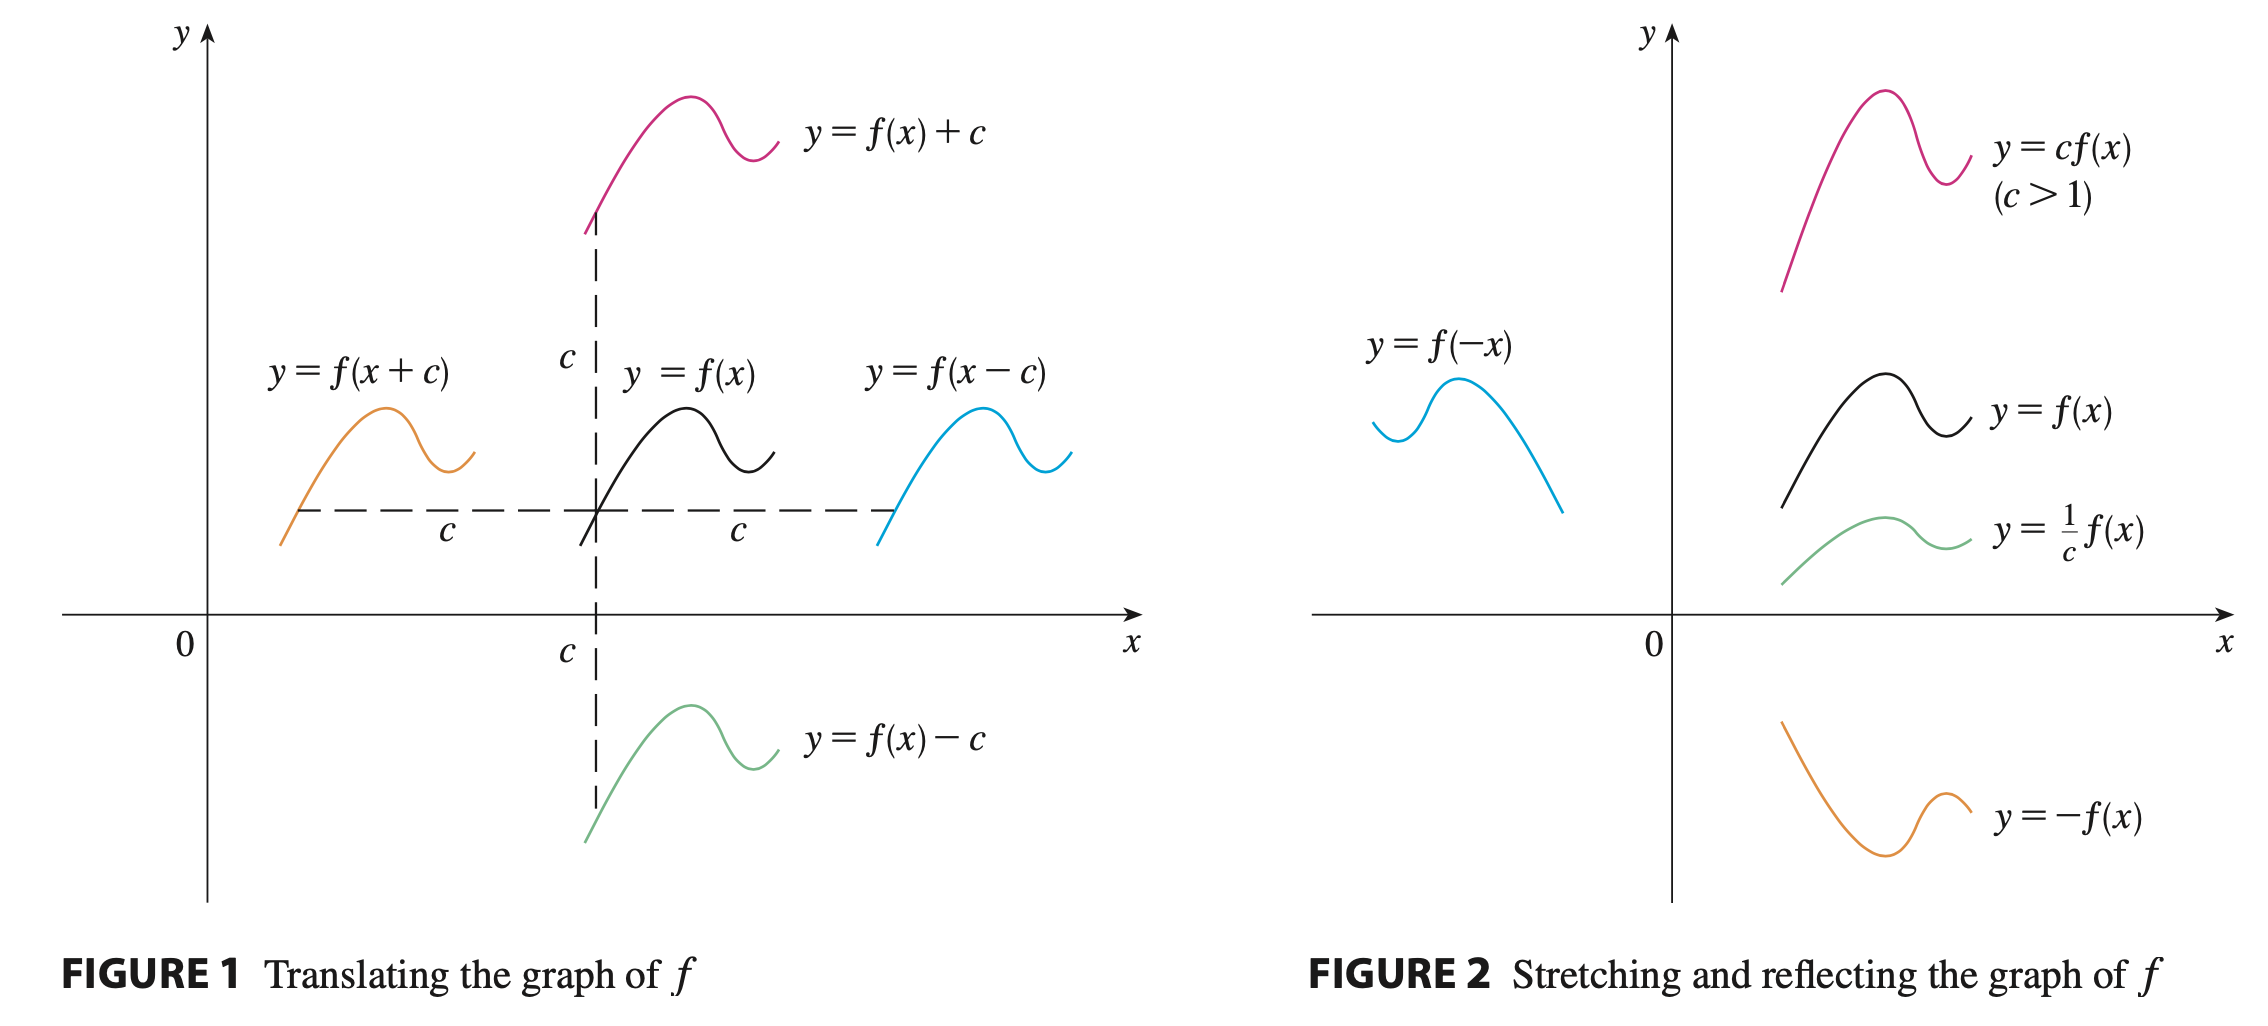
\includegraphics[scale=.3]{fig/transformations}}
\label{fig}
\end{figure}
\end{frame}

%\begin{frame}
%\newhead{Examples} Sketch the graphs given by
%\begin{enumerate}[<+->]
%\item[(a)] $y=\sqrt{2-x}$
%\item[(b)] $y=3\sin(2x+\pi)$
%\end{enumerate}
%\end{frame}

\end{document}